\section{Dynamic Bayesian networks}
\label{sec:dbn}

A Bayesian network is a graphical model that represents random variables and
their dependencies on eachother (see figure~\ref{fig:bn}). Each random variable
corresponds to a node and a directed edge represents a dependency between the
target and the source node. \parencite{heckerman1998tutorial}. For instance in
figure~\ref{fig:bn}, $Z$ depends on the setting of $X$ and $Y$. 

\begin{figure}[H]
\centering
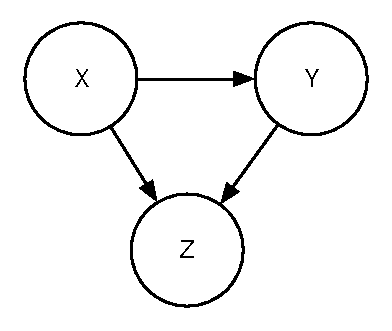
\includegraphics[width=0.4\textwidth]{images/BN.pdf}
\caption{A simple Bayesian network}
\label{fig:bn}
\end{figure}

A dynamic Bayesian network (DBN) is a Bayesian network where the random
variables are allowed to depend on prior settings of the same random variables
as well as eachother, see figure~\ref{fig:dbn}.

\begin{figure}[H]
    \centering
    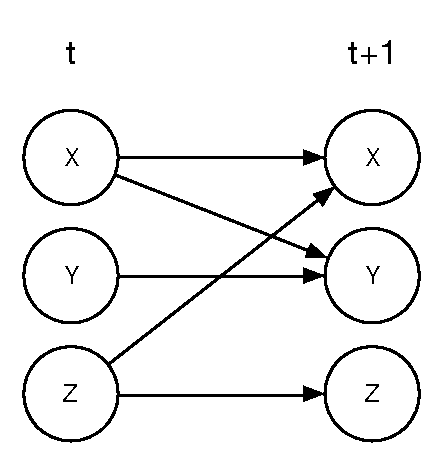
\includegraphics[width=0.5\textwidth]{images/DBN.pdf}
    \caption{A simple dynamic Bayesian network}
    \label{fig:dbn}
\end{figure}

In Bayesian networks as well as dynamic Bayesian networks one can define the
parents of a random variable to be the variables that it depends on. In the
Bayesian network in figure~\ref{fig:bn} the parents of $Z$ are $pa(Z) = \{X,
Y\}$ and in figure~\ref{fig:dbn} the parents of $Y$ are $pa(Y_{t+1}) = \{Y_t,
X_t\}$.

States in an MDP can be factored into several state variables representing
different features of the state. Using this factorisation transition
probabilities can be represented by a set of Bayesian networks, one network for
each possible action. 

In each network every state variable, $n_i$, is a node representing the setting
at time $t$, as well as a node, $n_i'$, representing setting at time $t+1$. If
the probability distribution of a certain state variable $n_k'$ is affected by
the value of another state variable $n_j$ if action $a$ is taken then there is
a directed edge from $n_j$ to $n_k'$ in the DBN corresponding to action $a$
\parencite{guestrin2003efficient}.
